\TODO{still lacks better intros}
% problem intro
Currently an architect starts the building design work flow by drawing rough
free form sketches of the desired building. These drawings are highly subjective
and clients have a hard time in their interpretation and validation.
The information captured in such drawings has little use in the remaining stages
of building design.

\TODO{insert draft sketches}

There are systems which are commonly used for professional building layouts
such as Autodesk Autocad \cite{SITE-AUTOCAD}.
The architect replicates his former ideas in the rigid standardized interface
offered by these systems. This is a rigorous endeavor, taking much time to be asserted.

After the main project documents are issued comes the time when the idea has to be pitched to end clients.
In order to gather buyers and investors its common to generate colorful previews of the building featuring increasingly realistic features such as detailed materials, light propagation and crowd simulations.
See Fig. \ref{FIG-REALISTIC}.

\begin{figure}[!ht]
	\centering
	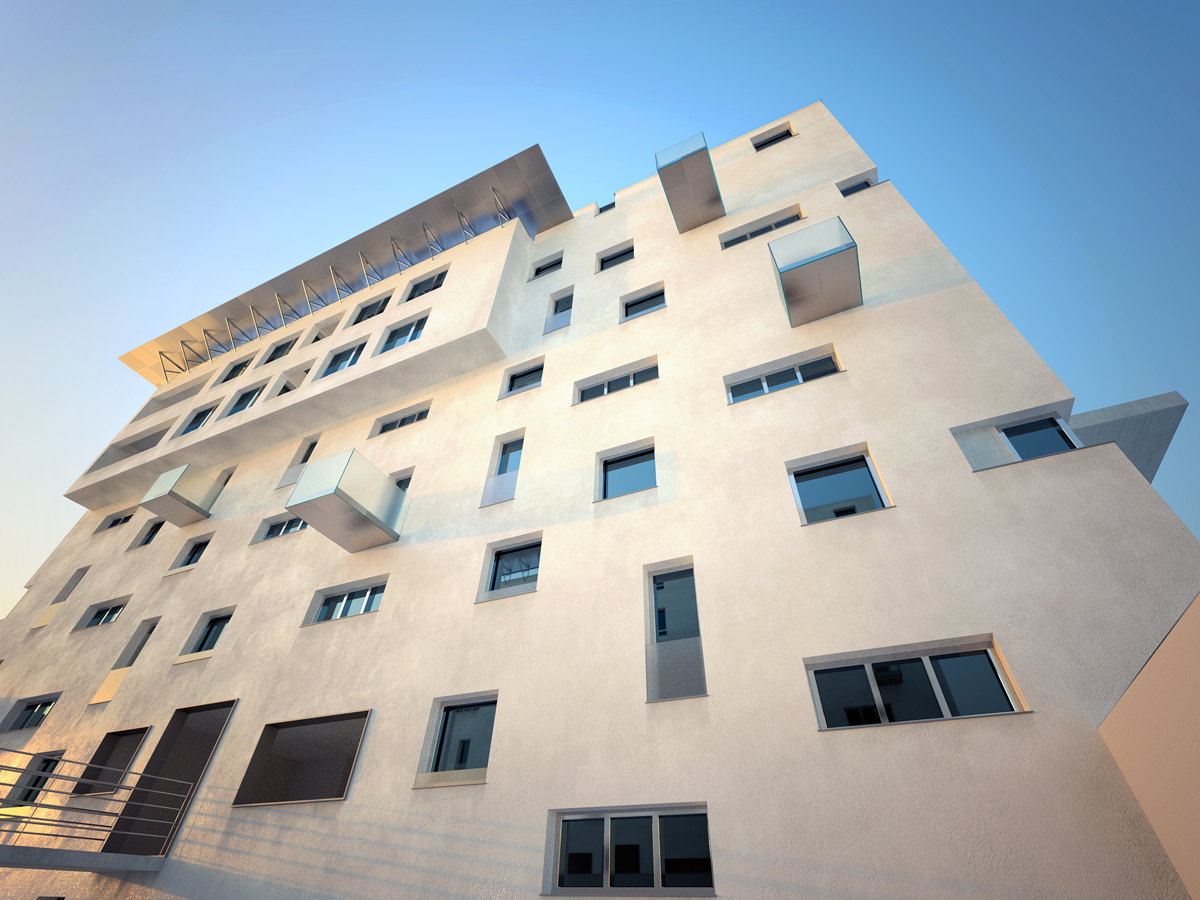
\includegraphics[width=6cm]{gfx/realistic01.jpg}
	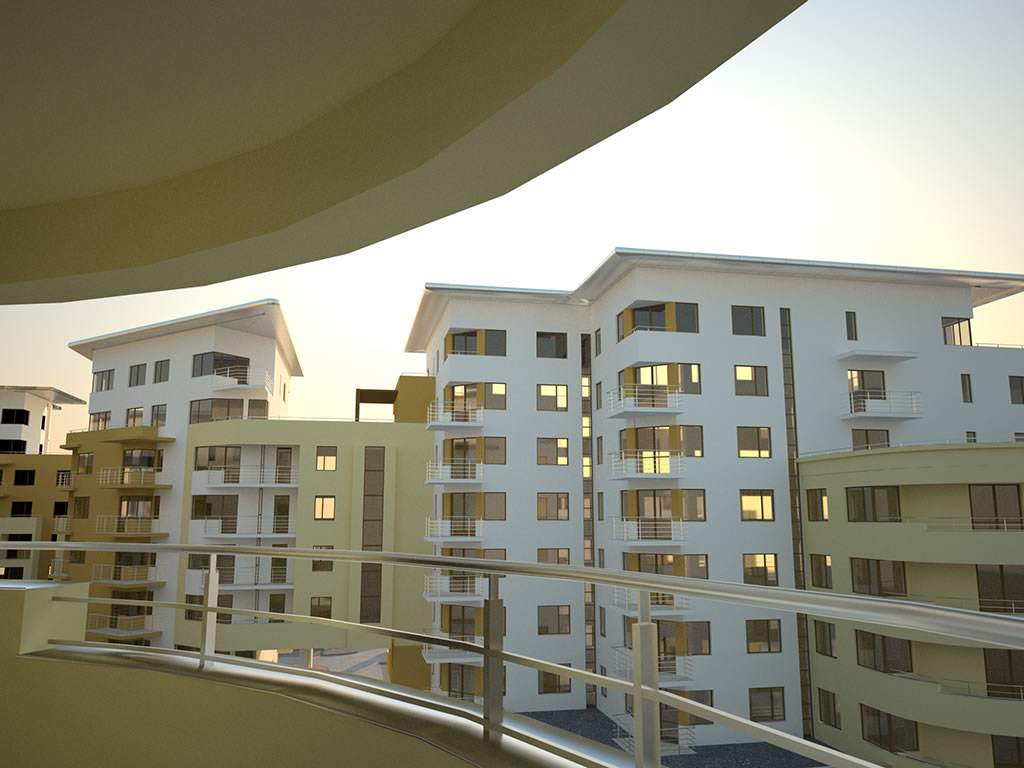
\includegraphics[width=6cm]{gfx/realistic03.jpg}
	\caption{Realistic renderings done with Maxwell Renderer}
	\label{FIG-REALISTIC}
\end{figure}

% 3 stage process
\TODO{Redo workflow figures}
Despite the ongoing advances in computation, the architectural workflow keeps these three separated stages
that don't share media or applications.% (Fig. \ref{FIG-WORKFLOW1}).
Both the conceptual design stage and the final reviewing and marketing stage would benefit from 
an integrated system with a comprehensive set of design actions
and good navigation and content reviewing capabilities.

%\begin{figure}[!ht]
%	\centering
%	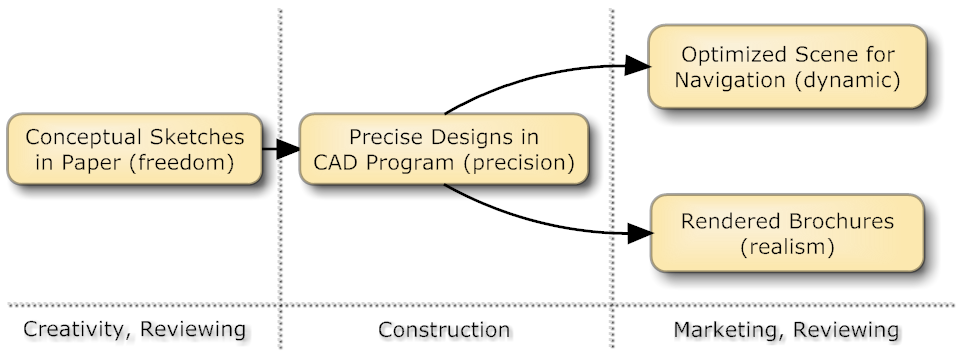
\includegraphics[width=12cm]{gfx/workflow1.png}
%	\caption{Architectural project work flow}
%	\label{FIG-WORKFLOW1}
%\end{figure}

% remote and multi-user reviews - costs and cycle
The possibility to make part of a review session remotely can benefit both parts:
it is more cost-effective for the architects than hosting each review event and
it allows a shorter reviewing cycle, 

% merge with environment and experiment more
The architect can benefit from the system by being able to experiment different locations
for the building and obtain a better integration between the new design and its surroundings.

% constraints to the architect
In order for an architect to use a computer program for drawing early designs,
it must be flexible enough not to limit the architect in expressing his vision.
Most current systems constrain architect's creativity \cite{TOW3D}.

% constraints to the client



% multimodal int.
A set of input and output modalities must be assembled and orchestrated

 must then be assembled with the purpose of offering
the users an immersive experience. Therefore this set must be chosen and
means must be given to users to allow them to perform actions like walking or creating
annotations.

% navigation, multi user
Having also the purpose of client reviewing and showcasing of designs,
the system should offer a comprehensive interface,
one that aids the user in navigating the world with a gentle learning curve.
Reviewing could also be done remotely.
Either in a local or remote set, the system should allow
concurrent browsing and editing of the world.


